\documentclass[a4paper,12pt]{article}
\usepackage[left=1in,right=1in,top=1in,bottom=1in]{geometry}
\usepackage{graphicx}
\usepackage{hyperref}
\setlength{\parindent}{0cm}
\title{Anushka S - ME20B029}
\author{}
\date{June 29,2021}
\begin{document}
\maketitle
\section{Biot-Savart law}
The Biot–Savart law is an equation describing the magnetic field generated by a constant electric current. It relates the magnetic field to the magnitude, direction, length, and proximity of the electric current. The Biot–Savart law is fundamental to magnetostatics, playing a role similar to that of Coulomb's law in electrostatics.\cite{webref1}
\subsection{Equation:}
\begin{equation}
    {\LARGE{\textbf{$\vec{dB}=\frac{\mu_{0} I\vec{dl}\times\hat{r}}{4\pi r^2}$}}}
    \label{eqn}
\end{equation}
\subsection{Analysis:}
\begin{figure}[h]
	{\begin{center}
		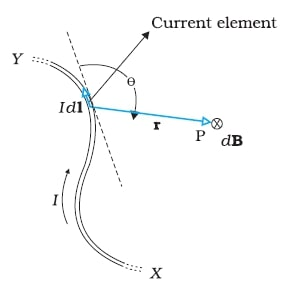
\includegraphics[scale=0.5]{ME20B029.jpg}
	\end{center}}
	\caption{A current element Idl produces a magnetic field at point P given by the Biot-Savart law \cite{picture}}
	\label{fig}
\end{figure}
Consider a wire carrying current I as shown in figure \ref{fig}. Equation \ref{eqn} gives the magnetic field {$\vec{dB}$} produced by an element {$\vec{dl}$} 
of the wire at the point P situated at a distance {\textbf{r}} from it. Here, {$\mu_{0}$} is the permeability of free space, and has value {$4\pi\times10^{-7}$}.\cite{webref2}
The magnitude of {$\vec{dB}$} is given by: 
\begin{equation}
{\LARGE{\textbf{${dB}=\frac{\mu_{0} Idlsin\theta}{4\pi r^2}$}}}
\end{equation}
\subsection{Applications}
The Biot–Savart law can be used in the calculation of magnetic responses even at the atomic or molecular level, e.g. chemical shieldings or magnetic susceptibilities, provided that the current density can be obtained from a quantum mechanical calculation or theory.The Biot–Savart law is also used in aerodynamic theory to calculate the velocity induced by vortex lines.\cite{webref1}

\bibliography{bibliography.bib}
\bibliographystyle{unsrt}
\end{document}
